%
% File acl2019.tex
%
%% Based on the style files for ACL 2018, NAACL 2018/19, which were
%% Based on the style files for ACL-2015, with some improvements
%%  taken from the NAACL-2016 style
%% Based on the style files for ACL-2014, which were, in turn,
%% based on ACL-2013, ACL-2012, ACL-2011, ACL-2010, ACL-IJCNLP-2009,
%% EACL-2009, IJCNLP-2008...
%% Based on the style files for EACL 2006 by 
%%e.agirre@ehu.es or Sergi.Balari@uab.es
%% and that of ACL 08 by Joakim Nivre and Noah Smith

\documentclass[11pt,a4paper]{article}
\usepackage[hyperref]{acl2019}
\usepackage{times}
\usepackage{latexsym}
\usepackage{graphicx}
\usepackage{amsmath}
\usepackage[utf8]{inputenc}
\usepackage{xspace}
\usepackage{paralist}
\usepackage{booktabs}
%\usepackage{pdfpages}

\usepackage{tikz}
\usepackage{tikz-qtree}

\usepackage{url}
\usepackage[normalem]{ulem}

\aclfinalcopy % Uncomment this line for the final submission
\def\aclpaperid{BlackboxNLP 31}  %  Enter the acl Paper ID here

%\setlength\titlebox{5cm}
% You can expand the titlebox if you need extra space
% to show all the authors. Please do not make the titlebox
% smaller than 5cm (the original size); we will check this
% in the camera-ready version and ask you to change it back.

\newcommand\BibTeX{B\textsc{ib}\TeX}
\newcommand\eg{e.g.\ }
\newcommand\ie{i.e.\ }
\newcommand\footurl[1]{\footnote{\url{#1}}}

% how to call the input and output positions
% input, i.e. attended to:
\newcommand{\word}{\emph{input state}\xspace}
\newcommand{\words}{\emph{input states}\xspace}
% output, i.e. they attend to input:
\newcommand{\state}{\emph{output state}\xspace}
\newcommand{\states}{\emph{output states}\xspace}

\def\RR#1{{\color{blue}RR: \it #1}}
\def\DM#1{{\color{red}DM: \it #1}}
\def\JL#1{{\color{magenta}JL: \it #1}}
\def\JLrepl#1#2{{\color{magenta}JL: \sout{#1} \it #2}}
\def\DEL#1{{\color{green}SMAZAT: \it #1}}
\def\REC#1{{\color{cyan}REC: \it #1}}
\def\JL#1{}
\def\JLrepl#1#2{}
\def\RR#1{}
\def\DM#1{}
\def\DEL#1{}

\title{}

\author{}

\date{}

\begin{document}
\maketitle
\begin{abstract}
\end{abstract}

\begin{figure}[t]
%\begin{center}
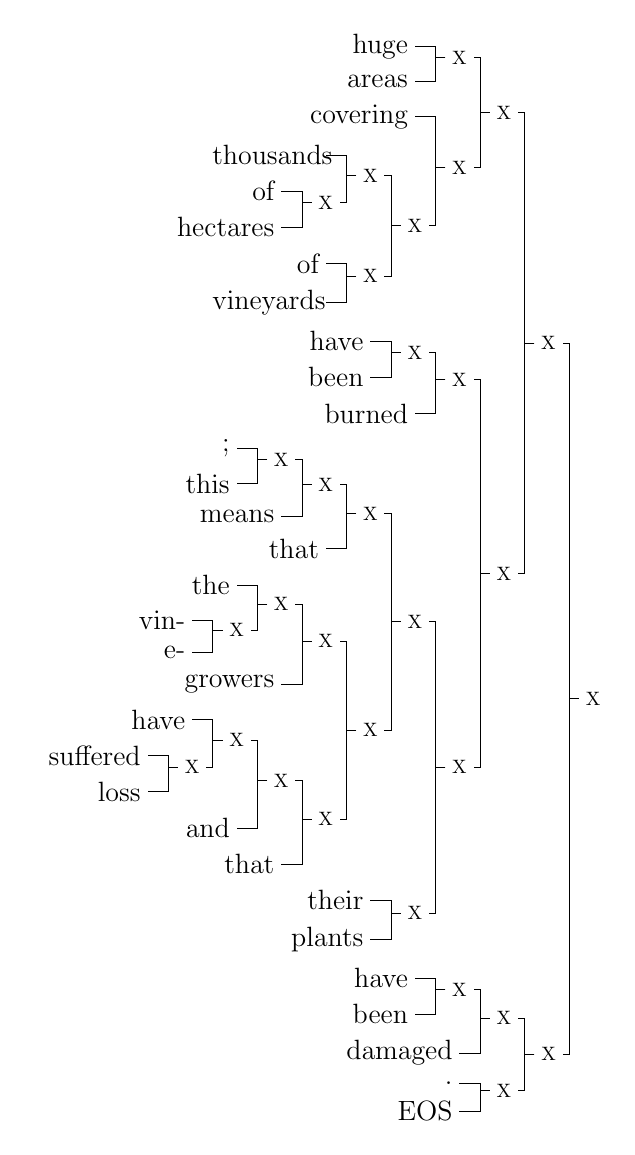
\begin{tikzpicture}[scale=0.7, grow=left]
\tikzset{every leaf node/.style={font=\Large, align=right, anchor=east, text width=55pt}}
\tikzset{level distance=23pt}
\tikzset{edge from parent/.style=
{draw,
edge from parent path={(\tikzparentnode.west)
-- +(-5pt, 0)
|- (\tikzchildnode.east)}}}
%\tikzset{sibling distance=5pt}
%\LARGE
\Tree
[.X
  [.X
    [.X
      [.X huge areas ]
      [.X covering [.X [.X thousands [.X of hectares ] ] [.X of vineyards ] ] ] ]
    [.X
      [.X [.X have been ] burned ]
      [.X
        [.X
          [.X [.X [.X ; this ] means ] that ]
          [.X
            [.X [.X the [.X vin- e- ] ] growers ]
            [.X [.X [.X have [.X suffered loss ] ] and ] that ] ] ]
        [.X their plants ] ] ] ]
  [.X [.X [.X have been ] damaged ] [.X . EOS ] ] ]
\end{tikzpicture}
%\end{center}
\caption{A constituency tree generated by our tree extraction algorithm from the attention matrices of the en-de encoder for the 4th sentence of the evaluation set.
%(The word ``vine-growers'' is split into 3 subwords.)
}
\label{fig:tree}
\end{figure}
\end{document}
